\documentclass[mathserif,professionalfont,hyperref={pdfpagelabels=false}]{beamer}
\usepackage{pxfonts} 
%\usepackage{eulervm}
\usepackage[english]{babel}
\usepackage{calc}
\usepackage[absolute,overlay]{textpos}
\mode<presentation>{\usetheme{tud}}
%\usepackage{subcaption}
\usepackage{tcolorbox}
\usepackage{tikz}
\usetikzlibrary{positioning,arrows}
\usepackage[utf8x]{inputenc}
\usepackage{scalefnt}
\usetikzlibrary{decorations.markings}
\usetikzlibrary{shapes,snakes}
\usetikzlibrary{shapes.geometric}
\usetikzlibrary{fit}					
\usetikzlibrary{backgrounds}
\usetikzlibrary{positioning}
\usetikzlibrary{arrows}
\usepackage{pgffor}
\usepackage{amsmath,amssymb,mathrsfs}
\usepackage{amsthm}
\usepackage{color}
\usepackage{wasysym}
\usepackage{pdfpages}
\usepackage{paralist}
\usepackage{framed}
\usepackage{fancybox} %kaders
\usepackage{pifont}
\usepackage{pgfplots}
\usepackage{listofsymbols}
\usepackage{multirow}
\usepackage{appendixnumberbeamer}
\usepackage[scaled]{helvet}
\usepackage[round]{natbib}
\tikzstyle{every picture}+=[remember picture]
\tikzstyle{na} = [baseline=-.5ex]


\title[Accuracy of original MPM]{Accuracy of original MPM}
%\institute[]{}
\author[]{Lisa Wobbes, Roel Tielen}
\date[\today]{\today}

\definecolor{blueM}{rgb}{0.4, 0.6, 0.8}


\begin{document}
%titel----------------------------------------------------------------------------------------------------------------------------------------------------------------
{
%\usebackgroundtemplate{\includegraphics[width=\paperwidth,height=\paperheight]{logos}}%
%\setbeamertemplate{footline}{\usebeamertemplate*{minimal footline}}
\frame{\titlepage}
}

%outline------------------------------------------------------------------------------------------------------------------------------------------------------------
\begin{frame}{Outline}
\begin{itemize}
\item ``Original'' MPM
\item Numerical accuracy
\item Benchmarks
	\begin{itemize}
	\item Vibrating bar 
	%\item Vibrating hyper-elastic bar
	\item Oedometer
	\end{itemize}
\item Sources of spatial errors
\begin{itemize}
\item Analogy with FEM
\item Grid crossing
\end{itemize}
\item Outlook
\end{itemize}
\end{frame}

%------------------------------------------------------------------------------------------------------------------
\begin{frame}{``Original'' MPM}
\begin{itemize}
\item Modified Lagrangian algorithm
\item Euler-Cromer time integration
\item Piecewise linear basis functions
\item No additional interventions
\pause
\item Own MATLAB implementation
\item 1D (UL)FEM/MPM 
\item Simplified version of Deltares' code
\end{itemize}
\end{frame}

%%------------------------------------------------------------------------------------------------------------------
%\begin{frame}{Numerical accuracy}
%\begin{tcolorbox}[colback=red!5,colframe=red!50!black,title=Numerical Approximation]
%$u_{ex} = u_{num} + \mathcal{O}(\Delta x^n) + \mathcal{O}(\Delta t^m)$ %with $n \leq 2$
%\end{tcolorbox}
%\begin{tcolorbox}[colback=red!5,colframe=red!50!black,title=RMS Error]
%$Error_{RMS} = \sqrt{\frac{1}{n_p} \sum_{p=1}^{n_p}\left(u_{num}(x_p,t) - u_{ex}(x_p,t)\right)^2}$
%\end{tcolorbox}
%\begin{tcolorbox}[colback=blue!5,colframe=blue!40!black,title=Accuracy in displacement]
%For $\Delta t \to 0$, the order of accuracy is equal to $n$, i.e. the reduction of $\Delta x$ by a factor of 2 decreases the RMS error by $2^n$.
%\end{tcolorbox}
%\end{frame}

%------------------------------------------------------------------------------------------------------------------
\begin{frame}{Numerical accuracy}
\begin{overlayarea}{\textwidth}{6cm}
\begin{tcolorbox}[colback=red!5,colframe=red!50!black,title=Numerical Approximation]
$u_{ex} = u_{num} + \mathcal{O}(\Delta x^n) + \mathcal{O}(\Delta t^m)$ %with $n \leq 2$
\end{tcolorbox}
\pause
\begin{tcolorbox}[colback=blue!5,colframe=blue!40!black,title=Example]
\begin{overlayarea}{\textwidth}{1.1cm}
\begin{tabular}{l l l}
$n$ & Grid size      & Error\\
     & $\Delta x$    & $E$\\

\only<2>{
1\hspace{0.115cm}     & $\Delta x/2$ & $E/2$\\
}
\only<3-4>{
2\hspace{0.01cm}    & $\Delta x /2$ & $E/4$ 
}
\end{tabular}
\end{overlayarea}
\end{tcolorbox}
\only<4>{
\begin{tcolorbox}[colback=red!5,colframe=red!50!black,title=RMS Error]
$Error_{RMS} = \sqrt{\frac{1}{n_p} \sum_{p=1}^{n_p}\left(u_{num}(x_p,t) - u_{ex}(x_p,t)\right)^2}$
\end{tcolorbox}
}
\end{overlayarea}
\end{frame}
%------------------------------------------------------------------------------------------------------------------
\begin{frame}{Numerical Accuracy}
\begin{tcolorbox}[colback=red!5,colframe=red!50!black,title=Temporal accuracy]
MPM is first order accurate in time, i.e. $m=1$. 
\end{tcolorbox}
\pause
\begin{tcolorbox}[colback=red!5,colframe=red!50!black,title=Spatial accuracy]
\begin{tabular}{l l}
\textbf{Order of spatial accuracy} & \textbf{Source}\\
& \\
 2 & \citet{gong, steffen}\\
& \\
 0.5 - 1 & \citet{tran}\\
& \\
 lack of spatial convergence & \citet{gong, steffen} \\
\end{tabular}
\end{tcolorbox} 
\end{frame}

%------------------------------------------------------------------------------------------------------------------
\begin{frame}{Vibrating bar}
  \begin{minipage}{\linewidth}
      \centering
      \begin{minipage}{0.45\linewidth}
              \definecolor{darkred}{cmyk}{0,0.9,0.9,0.2}
\definecolor{darkblue}{cmyk}{0.9,0.5,0.1,0.2}
\tikzset{
mystyle1/.style={
  rectangle,
  inner sep=0.05pt,
  text width=1mm,
  fill=black
  }
}

\tikzset{
mystyle2/.style={
  circle,
  inner sep=0.1pt,
  text width=2mm,
  fill=red!80
  }
}
\tikzstyle{myarrows}=[line width=0.4mm,draw=darkred,postaction={draw, line width=0.4mm, shorten >=3mm, -}]
\begin{figure}[H]
\centering
\begin{tikzpicture}[scale=0.48]
 %structure
 \draw[fill=black!25] (0.5,2) rectangle (6.5,2.55);
 \draw[fill=darkblue] (-0.3,3.5) rectangle (0.5,1);
%initial velocity
%\foreach \i in {1,2,3,4,5}
%{
%        \pgfmathsetmacro{\z}{0.5 + (6/5)*\i};
%        \pgfmathsetmacro{\y}{2.275};
%        \pgfmathsetmacro{\l}{1.1*sin((175*\z)/12)};
%        \draw[myarrows] (\z,\y) -- (\z+\l,\y);
%	\draw[->, ultra thick,darkred] (\z+1.01*\l,\y) -- (\z+1.05*\l,\y);
%}
%\draw (7.2,3.2) node {$v_0$};

\draw (7.2,3.2) node {$v_0$};
\draw[->, ultra thick,darkred] (6,2.275) -- (6.5+1.05*2,2.275);
%coordinate
\draw[->, thick] (-0.3,0.2)--(8.9,0.2);
\draw (8.5, -0.4) node {$x$};
 %coordinates
 \draw[thick] (0.5, 0.05)--(0.5,0.35);
 \draw (0.5,-0.4) node {0};
 \draw[thick] (6.5, 0.05)--(6.5,0.35);
 \draw (6.5,-0.4) node {$L$};
\end{tikzpicture}
\end{figure}
      \end{minipage}
      \hspace{0.01\linewidth}
      \begin{minipage}{0.45\linewidth}
         \begin{align}\nonumber
&\frac{\partial^2 u}{\partial t^2} = \frac{E}{\rho}\frac{\partial^2 u}{\partial x^2} \\ \nonumber
&\mbox{Boundary conditions: } \\  \nonumber
& u(0,t) = 0\\ \nonumber
& \frac{\partial u}{\partial x}(L,t) = 0\\  \nonumber
&\mbox{Initial conditions:}\\  \nonumber
& u(x,0) = 0\\ \nonumber
& \frac{\partial u}{\partial t}(x,0) = v_0\sin \left( \frac{\pi x}{2L} \right)
\end{align} 
      \end{minipage}
  \end{minipage}
\end{frame}
%------------------------------------------------------------------------------------------------------------------

\begin{frame}{Oedometer}
  \begin{minipage}{\linewidth}
      \centering
      \begin{minipage}{0.45\linewidth}
\definecolor{soil}{cmyk}{0,0.2,0.6,0.2}
\definecolor{darkred}{cmyk}{0,0.9,0.9,0.2}
\tikzset{
mystyle1/.style={
  rectangle,
  inner sep=0.05pt,
  text width=1mm,
  fill=black
  }
}

\tikzset{
mystyle2/.style={
  circle,
  inner sep=0.1pt,
  text width=2mm,
  fill=red!80
  }
}
\tikzstyle{myarrows}=[line width=0.4mm,draw=darkred,postaction={draw, line width=0.4mm, shorten >=3mm, -}]
\begin{figure}[h]
\centering
\begin{tikzpicture}
 %structure
 \draw[fill=black] (0.4,2.2) rectangle (2.6,-1.1);
 \draw[fill=soil] (0.5,2) rectangle (2.5,-1);
 \draw[fill=black!25] (0.5,2) rectangle (2.5,2.35);
 \draw (1.5, 0.5) node {soil};

 %load
 \draw[myarrows] (0.7,3) -- (0.7,2.35);
 \draw[myarrows] (1.5,3) -- (1.5,2.35);
 \draw[myarrows] (2.3,3) -- (2.3,2.35);
\draw[->, ultra thick,darkred] (0.7,2.35) -- (0.7,2.34);
\draw[->, ultra thick,darkred] (1.5,2.35) -- (1.5,2.34);
\draw[->, ultra thick,darkred] (2.3,2.35) -- (2.3,2.34);
 \draw (1.55,3.3) node {$p_0$};
%coordinate axis
\draw[->, thick] (-1,-1.2)--(-1,3.3);
\draw (-1.3, 3.1) node {$y$};
 %coordinates
\draw[thick] (-1.1,2)--(-0.9,2); 
\draw (-1.3,2) node {$H$};
\draw[thick] (-1.1,-1)--(-0.9,-1);
\draw (-1.3,-1) node {0};
\end{tikzpicture}
\end{figure}
      \end{minipage}
      \hspace{0.01\linewidth}
      \begin{minipage}{0.45\linewidth}
         \begin{align}\nonumber
&\frac{\partial^2 u}{\partial t^2} = \frac{E}{\rho} \frac{\partial^2 u}{\partial^2 y} -g \\ \nonumber
&\mbox{Boundary conditions: } \\  \nonumber
& u(0,t) = 0\\ \nonumber
& \frac{\partial u}{\partial y}(H,t) = \frac{p_0}{E} \\ \nonumber
&\mbox{Initial conditions:}\\  \nonumber
& u(y,0) = 0\\ \nonumber
& \frac{\partial u}{\partial t}(y,0) = 0
\end{align} 
      \end{minipage}
  \end{minipage}
\end{frame}
%---------------------------------------------------------------------------------------------------------------------
\begin{frame}{Accuracy: vibrating bar}
\begin{overlayarea}{\textwidth}{6cm}
\begin{center}
\only<1>{
\begin{figure}
\centering
\begin{tikzpicture}[scale=0.9]
\begin{axis}[
	%xlabel=$\log_2$(number of elements) ,
        xlabel=number of elements ,
        xmode=log,
        log basis x={2},
        xtick = {4,8,16,32,64},
       % xticklabels={2,3,4,5,6},
	xticklabels={4,8,16,32,64},
        ylabel=$\log_2$(RMS error), 
        ymode=log,
        log basis y={2},
	ytick = {0.001953125, 4.8828125e-04, 1.220703125e-04,3.0517578125e-05, 7.62939453125e-06,1.9073486328125e-06},
%         ytick = {2^{-9},2e-11,2e-13,2e-15,2e-15,2e-17,2e-19},
         yticklabels={-9,-11,-13,-15,-17,-19}
]
%\addplot coordinates { 
%  (4,  5.3698e-04) 
%  (8,  1.3456e-04)
%  (16, 3.3657e-05)
%  (32, 8.4138e-06)
%  (64, 2.1019e-06)
%  };

\addplot[color=red, mark=*] coordinates { 
  (4,  1.2918e-03) 
  (8,  3.2595 e-04)
  (16, 8.1795e-05)
  (32, 2.0632e-05)
  (64, 5.4969e-06)
  };
  
\addplot[color=black,mark=triangle*] coordinates { 
  (4,  1.0374e-03) 
  (8,  2.6167e-04)
  (16, 6.5694e-05)
  (32, 1.6625e-05)
  (64, 4.5505e-06)
  };  
\legend{MPM(1), MPM(4)} 
\end{axis}
%\end{semilogyaxis} 
\end{tikzpicture}
\end{figure}
}
\only<2>{
\begin{figure}
\centering
\begin{tikzpicture}[scale=0.9]
\begin{axis}[
        %xlabel=$\log_2$(number of elements) ,
	xlabel=number of elements ,
        xmode=log,
        log basis x={2},
        xtick = {4,8,16,32,64, 128},
	%xticklabels={2,3,4,5,6,7},
        xticklabels={4,8,16,32,64, 128},
        ylabel=$\log_2$(RMS error), 
        ymode=log,
        log basis y={2},
	ytick = {0.001953125, 4.8828125e-04, 1.220703125e-04,3.0517578125e-05, 7.62939453125e-06,1.9073486328125e-06, 4.768371582031250e-007},
%         ytick = {2^{-9},2e-11,2e-13,2e-15,2e-15,2e-17,2e-19},
         yticklabels={-9,-11,-13,-15,-17,-19,-21}
]
%\addplot coordinates { 
%  (4,  5.3698e-04) 
%  (8,  1.3456e-04)
%  (16, 3.3657e-05)
%  (32, 8.4138e-06)
%  (64, 2.1019e-06)
%  };

\addplot[color=red, mark=*] coordinates { 
  (4,  1.2918e-03) 
  (8,  3.2595 e-04)
  (16, 8.1795e-05)
  (32, 2.0632e-05)
  (64, 5.4969e-06)
  (128, 2.1502e-06) 
  };
  
\addplot[color=black,mark=triangle*] coordinates { 
  (4,  1.0374e-03) 
  (8,  2.6167e-04)
  (16, 6.5694e-05)
  (32, 1.6625e-05)
  (64, 4.5505e-06)
  (128, 1.9769e-06) 
  };  
\legend{MPM(1), MPM(4)} 
\end{axis}
%\end{semilogyaxis} 
\end{tikzpicture}
\end{figure}
}
\end{center}
\end{overlayarea}
\end{frame}



%------------------------------------------------------------------------------------------------------------------
\begin{frame}{Accuracy: oedometer}
  \begin{minipage}{\linewidth}
      \centering
      \begin{minipage}{0.42\linewidth}
	\begin{tcolorbox}[colback=red!5,colframe=red!50!black,title=Richardson's extrapolation]
	\small{The order of accuracy $n$ is obtained from $$\frac{u_{num}(2h)-u_{num}(4h)}{u_{num}(h)-u_{num}(2h)} = 2^{n}.$$}
	\end{tcolorbox}
	\only<2>{
	\begin{tcolorbox}[colback=blue!5,colframe=blue!40!black,title=Conclusion]
	\small{Lack of spatial convergence.}
	\end{tcolorbox}
	}
      \end{minipage}
    \hspace{0.01\linewidth}
      \begin{minipage}{0.48\linewidth}
      \: \:
      \:
      \:
      \:
      \: 
            \: \:
      \:
      \:
      \:
      \:
                  \: \:


       \begin{overlayarea}{\textwidth}{6cm}
      \only<1-2>{
      \centering
      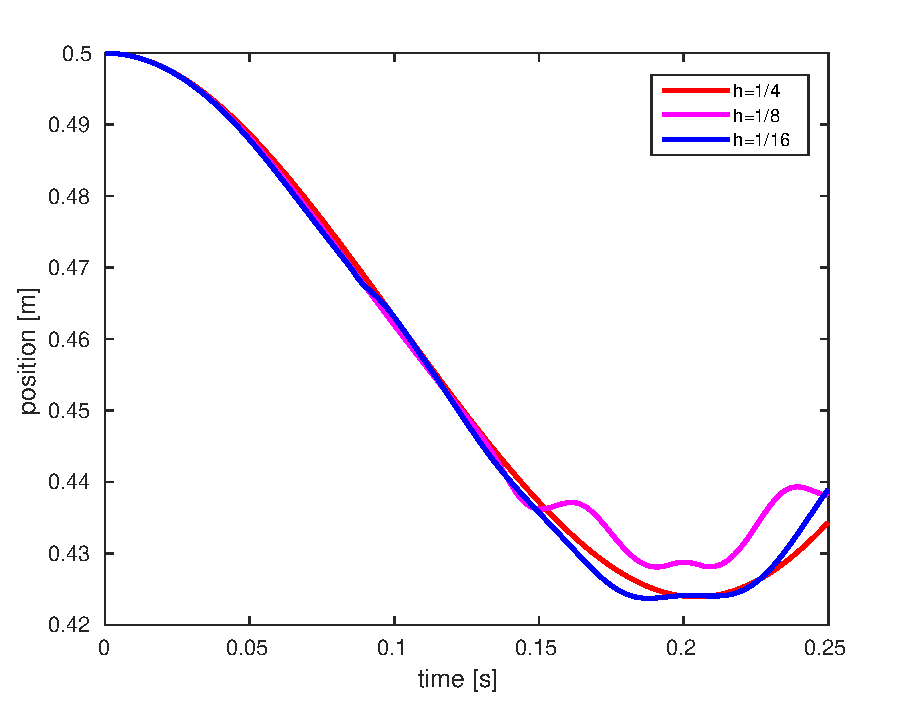
\includegraphics[scale=0.42]{images/accuracy_oedometer_langer}
      }
\end{overlayarea}
      \end{minipage}
  \end{minipage}
\end{frame}


%------------------------------------------------------------------------------------------------------------------

% \begin{frame}{Accuracy: oedometer}
% \begin{tcolorbox}[colback=blue!5,colframe=blue!40!black]
% Lack of convergence
% \end{tcolorbox}
% \begin{tcolorbox}[colback=red!5,colframe=red!50!black,title=Richardson's extrapolation]
% The order of accuracy $n$ is obtained from $$\frac{u_{num}(2h)-u_{num}(4h)}{u_{num}(h)-u_{num}(2h)} = 2^{n}.$$
% \end{tcolorbox}
% \end{frame}
% 
% %------------------------------------------------------------------------------------------------------------------
% \begin{frame}{Accuracy: oedometer}
% 
% \begin{overlayarea}{\textwidth}{6cm}
% \only<1>{
% \centering
% 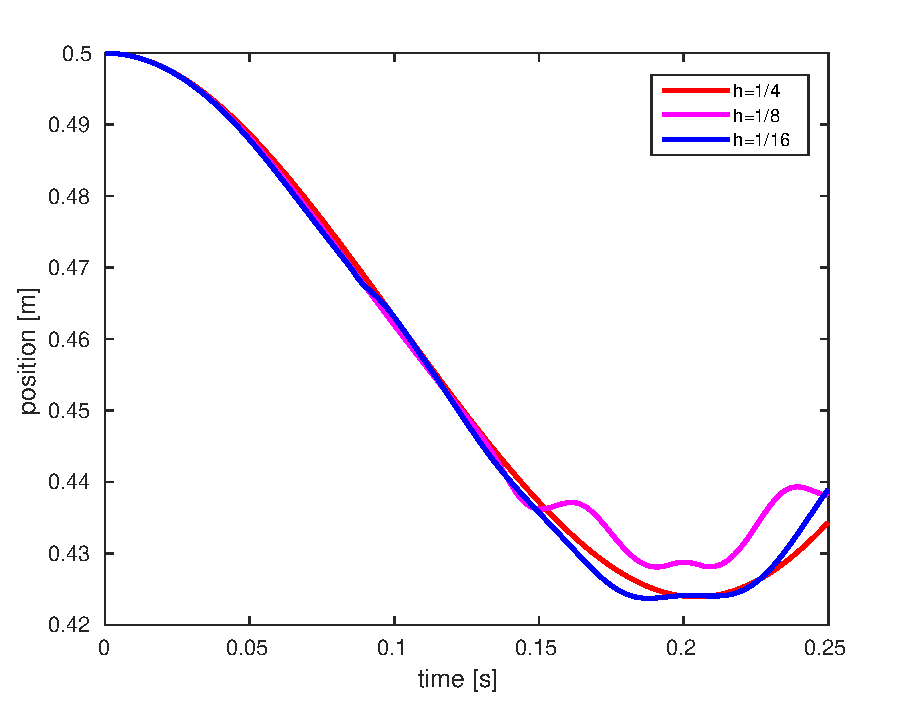
\includegraphics[scale=0.55]{images/accuracy_oedometer_langer}
% }
% \only<2>{
% \centering
% 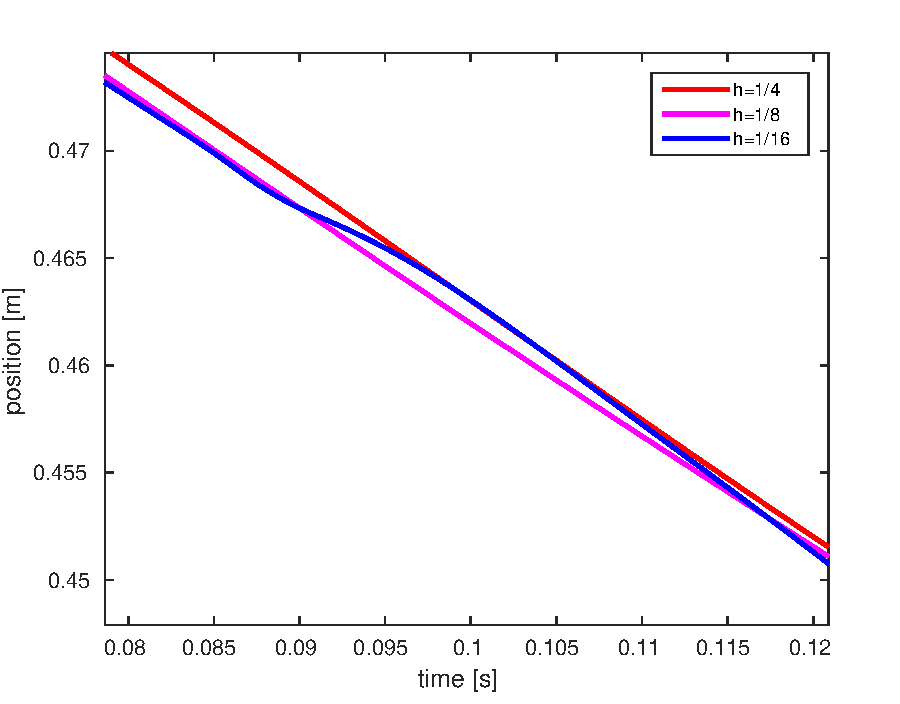
\includegraphics[scale=0.55]{images/accuracy_oedometer_zoomed}
% }
% \end{overlayarea}
% \end{frame}
%------------------------------------------------------------------------------------------------------------------
\begin{frame}{FEM: oedometer}
	\begin{tcolorbox}[colback=red!5,colframe=red!50!black,title=Theoretical order of accuracy]
	$k+1$, where $k$ is the order of the interpolating polynomials\footnotemark.
	\end{tcolorbox}
	\pause
	\begin{tcolorbox}[colback=blue!5,colframe=blue!40!black,title=Observations]
	\begin{itemize}
	 \item Lack of spatial convergence
	 \item Problems arise due to external forces\\
	 \begin{align}\nonumber
	 & \mathbf{M}\frac{d \mathbf{v}}{dt} = \mathbf{F}_{ext}-\mathbf{F}_{int},\\ \nonumber
	 & \mbox{where } \mathbf{F}_{ext} = \mathbf{N}(H)^Tp_0 - \int_0^H \mathbf{N}^T\rho g dy
	 \end{align}
	 %\item Further research is required
	\end{itemize}

	\end{tcolorbox}
\footnotetext{\citet{kan}}
\end{frame}

%------------------------------------------------------------------------------------------------------------------
\begin{frame}{FEM: vibrating bar}
\begin{center}
\begin{figure}
\begin{tikzpicture}[scale=0.9]
\begin{axis}[
        xlabel=number of elements,
        xmode=log,
        log basis x={2},
        xtick = {4,8,16,32,64, 128},
        xticklabels={4,8,16,32,64, 128},
        ylabel=$\log_2$(RMS error), 
        ymode=log,
        log basis y={2},
	ytick = {0.001953125, 4.8828125e-04, 1.220703125e-04,3.0517578125e-05, 7.62939453125e-06,1.9073486328125e-06, 4.768371582031250e-007},
%         ytick = {2^{-9},2e-11,2e-13,2e-15,2e-15,2e-17,2e-19},
         yticklabels={-9,-11,-13,-15,-17,-19,-21}
]
\addplot[color=blue,mark=square*] coordinates { 
  (4,  5.3698e-04) 
  (8,  1.3456e-04)
  (16, 3.3657e-05)
  (32, 8.4138e-06)
  (64, 2.1019e-06)
  (128,5.2381e-07)
  };
  
\addplot[color=red, mark=*] coordinates { 
  (4,  1.2918e-03) 
  (8,  3.2595 e-04)
  (16, 8.1795e-05)
  (32, 2.0632e-05)
  (64, 5.4969e-06)
  (128, 2.1502e-06) 
  };
  
\addplot[color=black,mark=triangle*] coordinates { 
  (4,  1.0374e-03) 
  (8,  2.6167e-04)
  (16, 6.5694e-05)
  (32, 1.6625e-05)
  (64, 4.5505e-06)
  (128, 1.9769e-06) 
  };  
\legend{FEM, MPM(1), MPM(4)} 
\end{axis}
%\end{semilogyaxis} 
\end{tikzpicture}
\end{figure}
\end{center}
\end{frame}

%------------------------------------------------------------------------------------------------------------------
\begin{frame}{Grid-crossing}
\begin{center}
\begin{tikzpicture}[scale = 0.4]
\definecolor{darkblue}{cmyk}{0.9,0.1,0.1,0.2}

\draw (0,0) coordinate(a_1) -- (10,0) coordinate(a_2);
\draw (a_1) -- (20,0) coordinate (a_3);

\draw (0,-1) coordinate (b_1);
\draw (20,-1) coordinate (b_3);
\draw (10,-1) coordinate (b_2);

\draw (b_1) node[below] {$x_{i-1}$};
\draw (b_3) node[below] {$x_{i+1}$} ;
\draw (b_2) node[below] {$x_{i}$};

\node[draw,circle,inner sep=3pt,fill] at (a_1) {};
\node[draw,circle,inner sep=3pt,fill] at (a_2) {};
\node[draw,circle,inner sep= 3pt,fill] at (a_3) {};

\node[draw,circle,inner sep=2.5pt,fill, color =darkblue] at (4,0) {};
\node[draw,circle,inner sep=2.5pt,fill, color = red] at (7.5,0) {};
\node[draw,circle,inner sep=2.5pt,fill, color =darkblue] at (14.5,0) {};
\node[draw,circle,inner sep=2.5pt,fill, color =darkblue] at (17,0) {};

 \draw[-to] (8,1) to[bend left] (12,1);

\end{tikzpicture}
\end{center}
\vspace{0.7cm}
\begin{center}
\begin{tikzpicture}[scale = 0.4]
\definecolor{darkblue}{cmyk}{0.9,0.5,0.1,0.2}
\draw (0,0) coordinate(a_1) -- (10,0) coordinate(a_2);
\draw (a_1) -- (20,0) coordinate (a_3);

\draw (0,-1) coordinate (b_1);
\draw (20,-1) coordinate (b_3);
\draw (10,-1) coordinate (b_2);

\draw (b_1) node[below] {$x_{i-1}$};
\draw (b_3) node[below] {$x_{i+1}$} ;
\draw (b_2) node[below] {$x_{i}$};

\node[draw,circle,inner sep=3pt,fill] at (a_1) {};
\node[draw,circle,inner sep=3pt,fill] at (a_2) {};
\node[draw,circle,inner sep= 3pt,fill] at (a_3) {};

\node[draw,circle,inner sep=2.5pt,fill, color =darkblue] at (5,0) {};
\node[draw,circle,inner sep=2.5pt,fill, color = red] at (13,0) {};
\node[draw,circle,inner sep=2.5pt,fill, color =darkblue] at (15,0) {};
\node[draw,circle,inner sep=2.5pt,fill, color =darkblue] at (18.25,0) {};



\end{tikzpicture}
\end{center}
\end{frame}


%-------------------------------------------------------------------------------------------------------------------
\begin{frame}{Grid-crossing: properties of shape functions}
\begin{center}
\begin{tikzpicture}[scale=1.5]
\definecolor{darkblue}{cmyk}{0.9,0.5,0.1,0.2}
    % Draw axes
    \draw [-,thick] (0,1.3) node (yaxis) [left] {$N_i$}
        |- (4,0) node (xaxis) [right] {};
    % Draw two intersecting lines
    \draw (0,0) coordinate (a_1) -- (2,1) coordinate (a_2);
    \draw (2,1) coordinate (b_1) -- (4,0) coordinate (b_2);
    \draw (2,0) coordinate (b_3);
    \draw (0,-0.2) node[below] {$x_{i-1}$};
    \draw (2,-0.2) node[below] {$x_{i}$};
    \draw (4,-0.2) node[below] {$x_{i+1}$};
    
 \shade[bottom color=darkblue!10, top color=darkblue!80] (0,0) --(2,0) --(2,1);
 \shade[bottom color=darkblue!10, top color=darkblue!80] (4,0) --(2,0) --(2,1);

\node[draw,circle,inner sep=3pt,fill] at (b_3) {};
\node[draw,circle,inner sep=3pt,fill] at (b_2) {};
\node[draw,circle,inner sep=3pt,fill] at (a_1) {};

\draw[dashed] (yaxis |- b_1) node[left] {$1$}
        -| (xaxis -| b_1) node[below] {};

\end{tikzpicture}
\end{center}

\begin{center}
\begin{tikzpicture}[scale=1.5]
\definecolor{darkblue}{cmyk}{0.9,0.5,0.1,0.2}
 \shade[bottom color=darkblue!10, top color=darkblue!60] (0,0)rectangle +(2,1);
 \shade[top color=darkblue!10, bottom color=darkblue!60] (2,0) rectangle +(2,-1);
    % Draw axes
    \draw [-,thick] (0,-1.2) -- (0,1.2) node (yaxis) [left] {$\nabla N_i$}
        |- (4,0) node (xaxis) [right] {};

    % Draw two intersecting lines
    \draw (0,1) coordinate (a_1) -- (2,1) coordinate (a_2);
    \draw (2,-1) coordinate (b_1) -- (4,-1) coordinate (b_2);
    \draw (2,0) coordinate (b_3);

    \draw (-0.25,-0.2) node[below] {$x_{i-1}$};
    \draw (1.8,-0.2) node[below] {$x_{i}$};
    \draw (4.25,-0.2) node[below] {$x_{i+1}$};
    


\node[draw,circle,inner sep=3pt,fill] at (0,0) {};
\node[draw,circle,inner sep=3pt,fill] at (2,0) {};
\node[draw,circle,inner sep=3pt,fill] at (4,0) {};


\end{tikzpicture}
\end{center}


\end{frame}



%--------------------------------------------------------------------------------------------------------------------
\begin{frame}{Grid crossing: internal force}
\centering
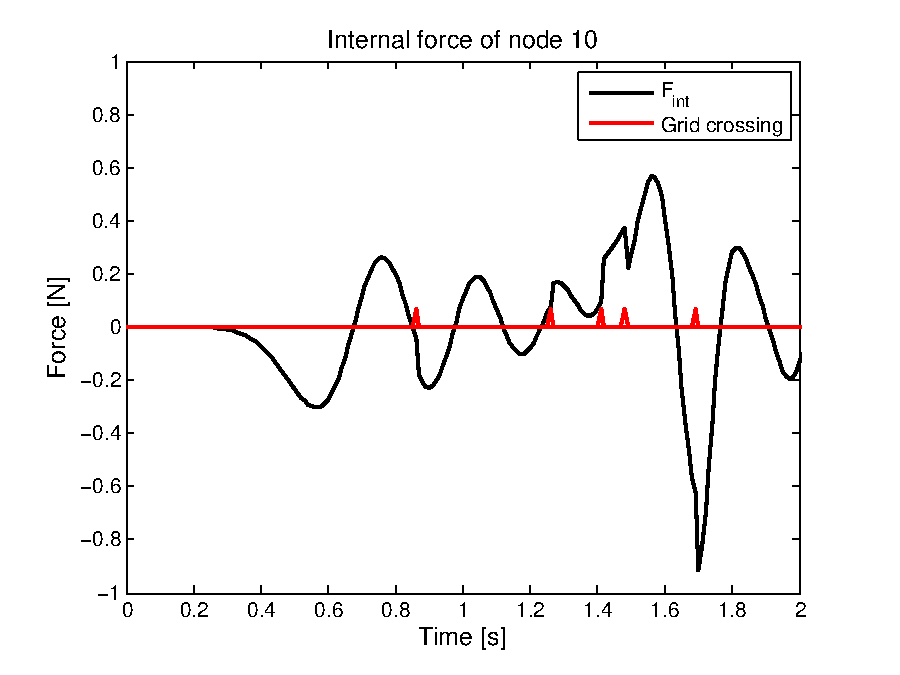
\includegraphics[width=0.7\paperwidth,height=0.7\paperheight]{images/Grid_crossing}
\end{frame}

%--------------------------------------------------------------------------------------------------------------------
\begin{frame}{Grid crossing: vibrating bar}
\begin{overlayarea}{\textwidth}{6cm}
\begin{center}
\only<1>{
\begin{figure}
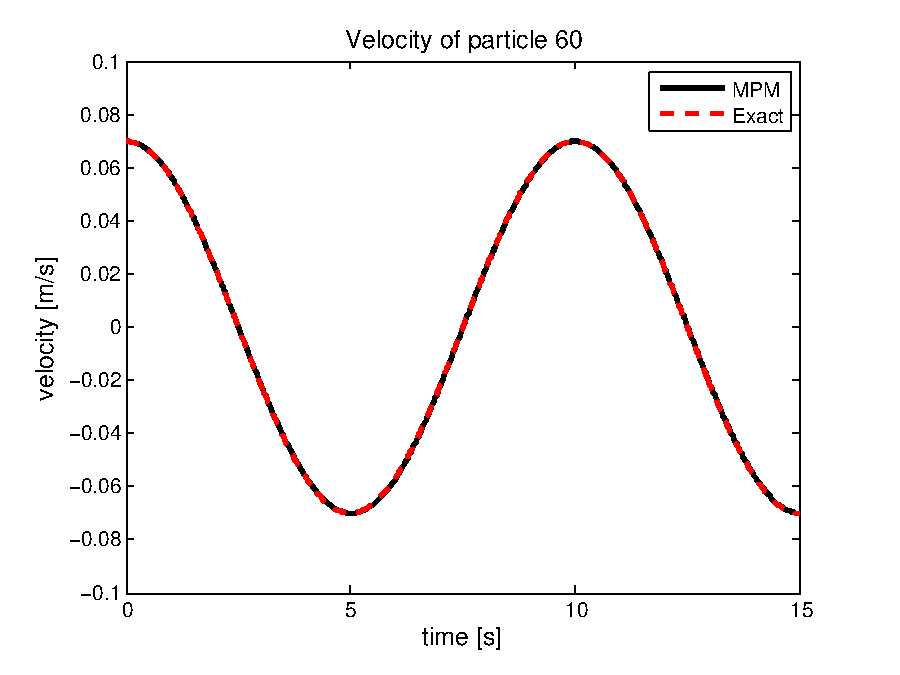
\includegraphics[scale=0.5]{images/vs_vel30}
\caption{\small{No grid crossing (30 elements).}}
\end{figure}
}
\only<2>{
\begin{figure}
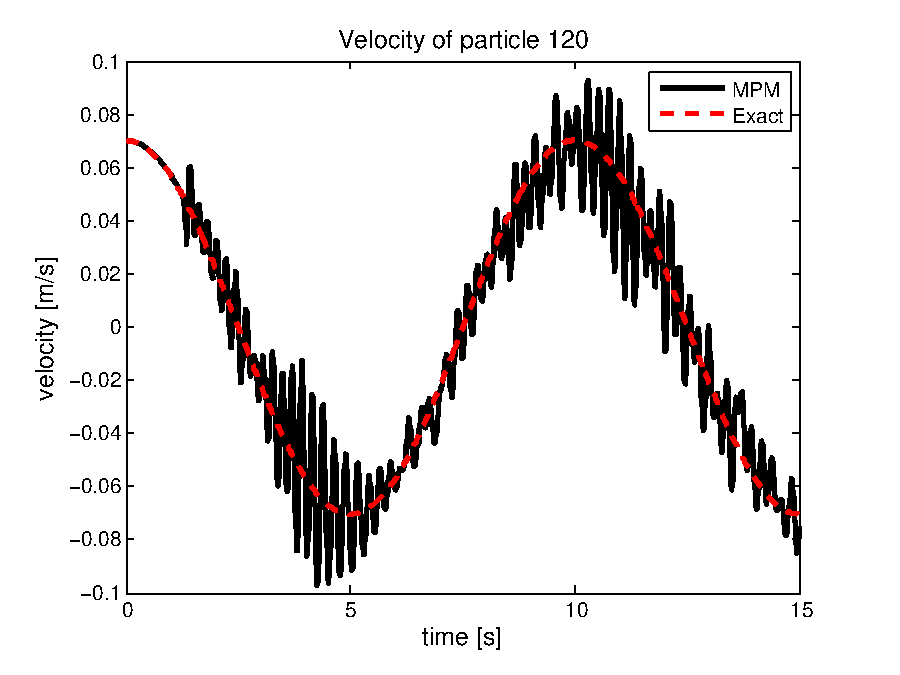
\includegraphics[scale=0.5]{images/vs_vel60}
\caption{\small{Grid crossing (60 elements).}}
\end{figure}
}
\end{center}
\end{overlayarea}
\end{frame}

% %--------------------------------------------------------------------------------------------------------------------
% \begin{frame}{Oedometer: position}
% \begin{figure}
% 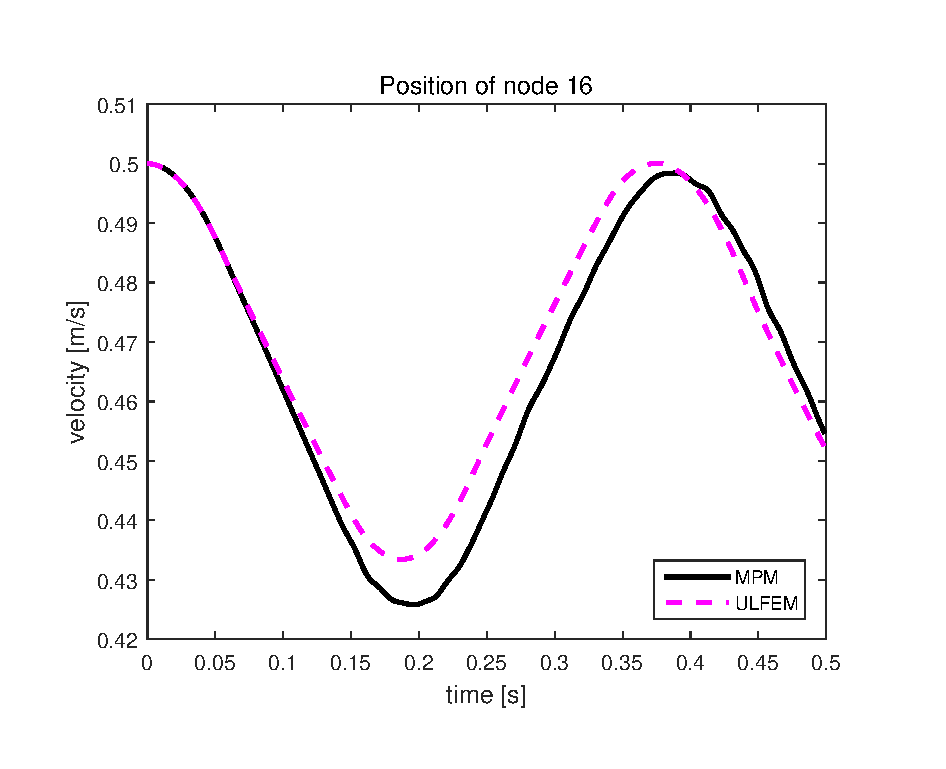
\includegraphics[scale=0.5]{images/oedometer_pos_30_10}
% %\caption{\small{Grid crossing (30 elements).}}
% \end{figure}
% \end{frame}

%--------------------------------------------------------------------------------------------------------------------
\begin{frame}{Grid crossing: oedometer}
\begin{figure}
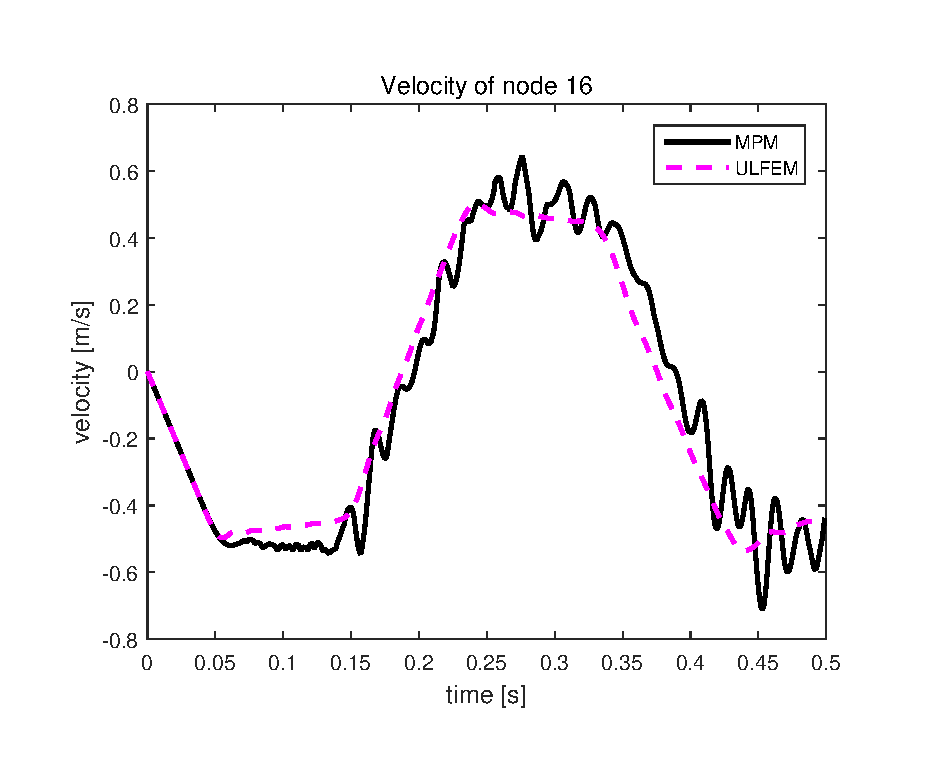
\includegraphics[scale=0.5]{images/oedometer_vel_30_10}
%\caption{\small{Grid crossing (30 elements).}}
\end{figure}
\end{frame}



%--------------------------------------------------------------------------------------------------------------------
\begin{frame}{Main sources of spatial errors}
\begin{tcolorbox}[colback=blue!5,colframe=blue!40!black,title=Presented today]
\begin{itemize}
\item Errors arising due to external forces
\item Grid crossing errors
\end{itemize}
\end{tcolorbox}
\begin{tcolorbox}[colback=red!5,colframe=red!50!black,title=Other sources\footnotemark]
\begin{itemize}
\item Mass mapping error
\item Momentum mapping error
\item Force mapping error
\end{itemize}
\end{tcolorbox}
\footnotetext{\citet{tran}}
\end{frame}

%------------------------------------------------------------------------------------------------------------------
\begin{frame}{Conclusions}
\begin{tcolorbox}[colback=blue!5,colframe=blue!40!black,title=Vibrating bar]
Second order accuracy: unless particles  cross element boundaries.
\end{tcolorbox}
\pause
\begin{tcolorbox}[colback=blue!5,colframe=blue!40!black,title=Oedometer]
Lack of convergence: due to external forces and grid crossing.
\end{tcolorbox}
\pause
\begin{tcolorbox}[colback=blue!5,colframe=blue!40!black,title=Both problems]
Other error sources can be involved.
\end{tcolorbox}
\end{frame}

%-------------------------------------------------------------------------------------------------------------------
\begin{frame}{Outlook}
\begin{itemize}
\item External forces: further analysis 
\pause
\item Other sources of spatial error
\pause
\item Higher order interpolation functions
\pause
\item 2D MPM code in MATLAB
\pause
\item Deltares' implementation: analysis and recommendations
\end{itemize}
\end{frame}


%--------------------------------------------------------------------------------------------------------------------

\begin{frame}{References}
\begin{thebibliography}{22}
 \bibitem[Gong (2015)]{gong} Gong M.
 \newblock {\em Improving the Material Point Method.}
 \newblock The University of New Mexico, July, 2015.
 \bibitem[Van Kan (2008)]{kan} Van Kan J., Segal A., Vermolen F. 
\newblock {\em Numerical methods in scientific computing.}
 \newblock Delft University of Technology, 2008.
 \bibitem[Steffen (2008)]{steffen} Steffen M., Kirby R. M., Berzins M. 
\newblock {\em Analysis and reduction of quadrature errors in the material point method (MPM).}
 \newblock International Journal for Numerical Methods in Engineering 76, pp. 922-946, 2008.
 \bibitem[Tran (2010)]{tran} Tran L.T., Kim J., Berzins M. 
\newblock {\em Solving time-dependent PDEs using the material point method, a case study from gas dynamics.}
 \newblock International Journal for Numerical Methods in Fluids 62, pp. 709-732, 2010.
\end{thebibliography}
\end{frame}






%%%%%%%%%%%%%%%%%%%%%%%%%%%%%%%%%%%%%%%%%%%%%%%%%
%%%%%%%%%%%%%%%%%%%%%%%%%%%%%%%%%%%%%%%%%%%%%%%%%
%%%%%%%%%%%%%%%%%%%%%%%%%%%%%%%%%%%%%%%%%%%%%%%%%

\appendix


%\begin{frame}{Main sources of spatial errors}
%\begin{tcolorbox}[colback=blue!5,colframe=blue!40!black,title=Presented today]
%\begin{itemize}
%\item Errors arising due to external forces
%\item Grid crossing errors
%\end{itemize}
%\end{tcolorbox}
%\begin{tcolorbox}[colback=red!5,colframe=red!50!black,title=Other sources]
%\begin{itemize}
%\item Mass mapping error
%\item Momentum mapping error
%\item Force mapping error
%\end{itemize}
%\end{tcolorbox}
%
%\end{frame}

%%%%%%%%%%%%%%%%%%%%%%%%%%%%%%%%%%%%%%%%%%%%%%%%%

\begin{frame}{Grid crossing: internal force}
 \begin{align}\nonumber
  & F^{int}_{i+1} \approx \sum_{p=1}^{n_i} \nabla N_i(\xi_p)\sigma_p \Omega_p + \sum_{p=1}^{n_{i+1}}\nabla N_i(\xi_p) \sigma_p \Omega_p\\ \nonumber
  & F^{int}_{i+1} \approx \sigma \Omega (n_i - n_{i+1})\\ \nonumber
  & \: \\ \nonumber
  & \begin{cases}F^{int}_{i+1} = 0, &\mbox{if } n_{i} = n_{i+1} \\
\: \\
F^{int}_{i+1} \neq 0, & \mbox{otherwise} \end{cases}  
 \end{align}
\end{frame}
%%%%%%%%%%%%%%%%%%%%%%%%%%%%%%%%%%%%%%%%%%%%%%%%%
\begin{frame}{Depenence on PPC: vibrating string}
\begin{figure}
\begin{tikzpicture}[scale=0.9]
\begin{axis}[
        xlabel=number of elements,
        xmode=log,
        log basis x={2},
        xtick = {4,8,16,32,64, 128,256,512},
        xticklabels={4,8,16,32,64, 128,256,512},
        ylabel=$\log_2$(RMS error), 
        ymode=log,
        log basis y={2},
	ytick = {0.001953125, 4.8828125e-04, 1.220703125e-04,3.0517578125e-05, 7.62939453125e-06,1.9073486328125e-06},
%         ytick = {2^{-9},2e-11,2e-13,2e-15,2e-15,2e-17,2e-19},
         yticklabels={-9,-11,-13,-15,-17,-19}
]
\addplot[color=blue,mark=square*] coordinates { 
(4,1.037385e-03)
(8,2.616727e-04)
(16,6.569391e-05)
(32,1.662519e-05)
(64,4.550497e-06)
(128,1.976922e-06)
(256,5.355537e-06)
(512,1.847240e-05)
  };
  
\addplot[color=red, mark=*] coordinates { 
(4,9.917325e-04)
(8,2.501276e-04)
(16,6.280135e-05)
(32,1.590612e-05)
(64,4.383044e-06)
(128,2.983375e-06)
(256,7.372661e-06)
(512, 1.611112e-05)
  };
  
\addplot[color=black,mark=triangle*] coordinates { 
(4,9.667486e-04)
(8,2.438081e-04)
(16,6.121801e-05)
(32,1.551265e-05)
(64,4.252232e-06)
(128,3.928155e-06)
(256,8.992277e-06)
(512,1.168189e-05)
  };  
\legend{4 PPC, 6 PPC, 8 PPC} 
\end{axis}
%\end{semilogyaxis} 
\end{tikzpicture}
\end{figure}
\end{frame}

%%%%%%%%%%%%%%%%%%%%%%%%%%%%%%%%%%%%%%%%%%%%%%
\begin{frame}{Depenence on PPC: oedometer}
\begin{figure}
\pgfplotsset{every axis legend/.append style={
    at={(0.31,0.99)},
    anchor=north east}}
\begin{tikzpicture}[scale=0.9]
\begin{axis}[
        xlabel=number of elements,
        xmode=log,
        log basis x={2},
        xtick = {4,8,16,32,64, 128},
        xticklabels={4,8,16,32,64, 128},
        ylabel=$\log_2$(RMS error), 
        ymode=log,
        log basis y={2},
	ytick = {0.0078125, 0.001953125, 4.8828125e-04, 1.220703125e-04},
%         ytick = {2^{-9},2e-11,2e-13,2e-15,2e-15,2e-17,2e-19},
         yticklabels={-7,-9,-11,-13}
]
\addplot[color=blue,mark=square*] coordinates { 
(4, 0.0041)
(8, 0.0019)
(12, 7.7723e-04)
(16, 3.8530e-04)
(24, 3.5351e-04)
(32, 3.4308e-04)
(48, 0.0013)
(64, 0.0029)
(96, 0.0062)
(128,  0.0164)
  };
  
\addplot[color=red, mark=*] coordinates { 
(4,0.0040) 
(8,0.0018)  
(12,7.4299e-04) 
(16,3.7734e-04)  
(24,3.5202e-04)
(32, 5.8636e-04) 
(48,0.0028)   
(64,0.0025)
(96,0.0042)  
(128,0.0084)
  };
  
\addplot[color=black,mark=triangle*] coordinates { 
(4,0.0040) 
(8,0.0018)  
(12,7.2461e-04)
(16,3.7349e-04)  
(24,4.3493e-04)   
(32,0.0011)  
(48,0.0022)     
(64,0.0027)  
(96,0.0042)  
(128,0.0063)
};
\legend{4 PPC, 6 PPC, 8 PPC} 
\end{axis}
%\end{semilogyaxis} 
\end{tikzpicture}
\end{figure}
\end{frame}

%%%%%%%%%%%%%%%%%%%%%%%%%%%%%%%%%%%%%%%%%%%%%%%%%
\begin{frame}{Settings: vibrating bar}
\begin{table}[h]
\centering
\begin{tabular}{l | c c c}
 & Symbol & Value & Unit \\
\hline
Length& $L$ & 25 & m\\
Tension& $E$ & $ 100$ & Pa\\
Density & $\rho$ & $1$ & kg/m$^3$\\
Maximum velocity & $v_0$ & 0.1 & m/s\\
%Load & $p_0$ & $-5\cdot 10^3$ & Pa\\
%Gravitational acceleration & $g$ & 9.81 & m/s$^2$\\ 
Time step & $\Delta t$ &$ 1 \cdot10^{-3}$ & s\\
Measurement time$^1$ & $t$ & 0.5 & s\\
PPC$^2$ & & 4 & \\
\end{tabular}
\end{table}



\end{frame}

%%%%%%%%%%%%%%%%%%%%%%%%%%%%%%%%%%%%%%%%%%%%%%%%
\begin{frame}{Settings: oedometer}
\begin{table}[h]
\centering
\begin{tabular}{l | c c c}
 & Symbol & Value & Unit \\
\hline
Height & $L$ & 1 & m\\
Young's modulus& $E$ & $ 1 \cdot10^5$ & Pa\\
Density & $\rho$ & $1 \cdot10^3$ & kg/m$^3$\\
%Maximum velocity & $v_0$ & 0.1 & m/s\\
Load & $p_0$ & $0$ & Pa\\
Gravitational acceleration & $g$ & 9.81 & m/s$^2$\\ 
Time step & $\Delta t$ &$ 1 \cdot10^{-3}$ & s\\
Measurement time$^1$ & $t$ & 0.5 & s\\
Position particle$^1$ & $x_p$ & $\approx 0.5$ & m\\
Number of elements$^2$ & & 30& \\
PPC$^2$ & & 10 & \\
\end{tabular}
\end{table}
\end{frame}

%%%%%%%%%%%%%%%%%%%%%%%%%%%%%%%%%%%%%%%%%%%%%%%%
\begin{frame}{Settings: Steffen}
\begin{table}[h]
\centering
\begin{tabular}{l | c c c}
 & Symbol & Value & Unit \\
\hline
Length& $L$ & 1 & m\\
Tension& $E$ & $ 100$ & Pa\\
Density & $\rho$ & $100$ & kg/m$^3$\\
%Maximum velocity & $v_0$ & 0.1 & m/s\\
Load & $p_0$ & $0.7$ & Pa\\
Gravitational acceleration & $g$ & 0  & m/s$^2$\\ 
Time step & $\Delta t$ &$ 1 \cdot10^{-2}$ & s\\
Domain & & 1.15 & m \\
Number of elements & & 20& \\
PPC & & 10 & \\
\end{tabular}
\end{table}
\end{frame}

\end{document}